\documentclass[aspectratio=169]{beamer}
\setbeamertemplate{navigation symbols}{}
\usefonttheme{professionalfonts}
\usepackage{tikz}
\usetikzlibrary{positioning, arrows.meta}

\tikzset{
  alt/.code args={<#1>#2#3}{%
    \alt<#1>{\pgfkeysalso{#2}}{\pgfkeysalso{#3}}%
  }
}

\begin{document}

% ==========================================
% REVERSE MODE: GRADIENT FLOWING BACKWARD
% ==========================================
\begin{frame}[plain]
\centering
\resizebox{\textwidth}{!}{%
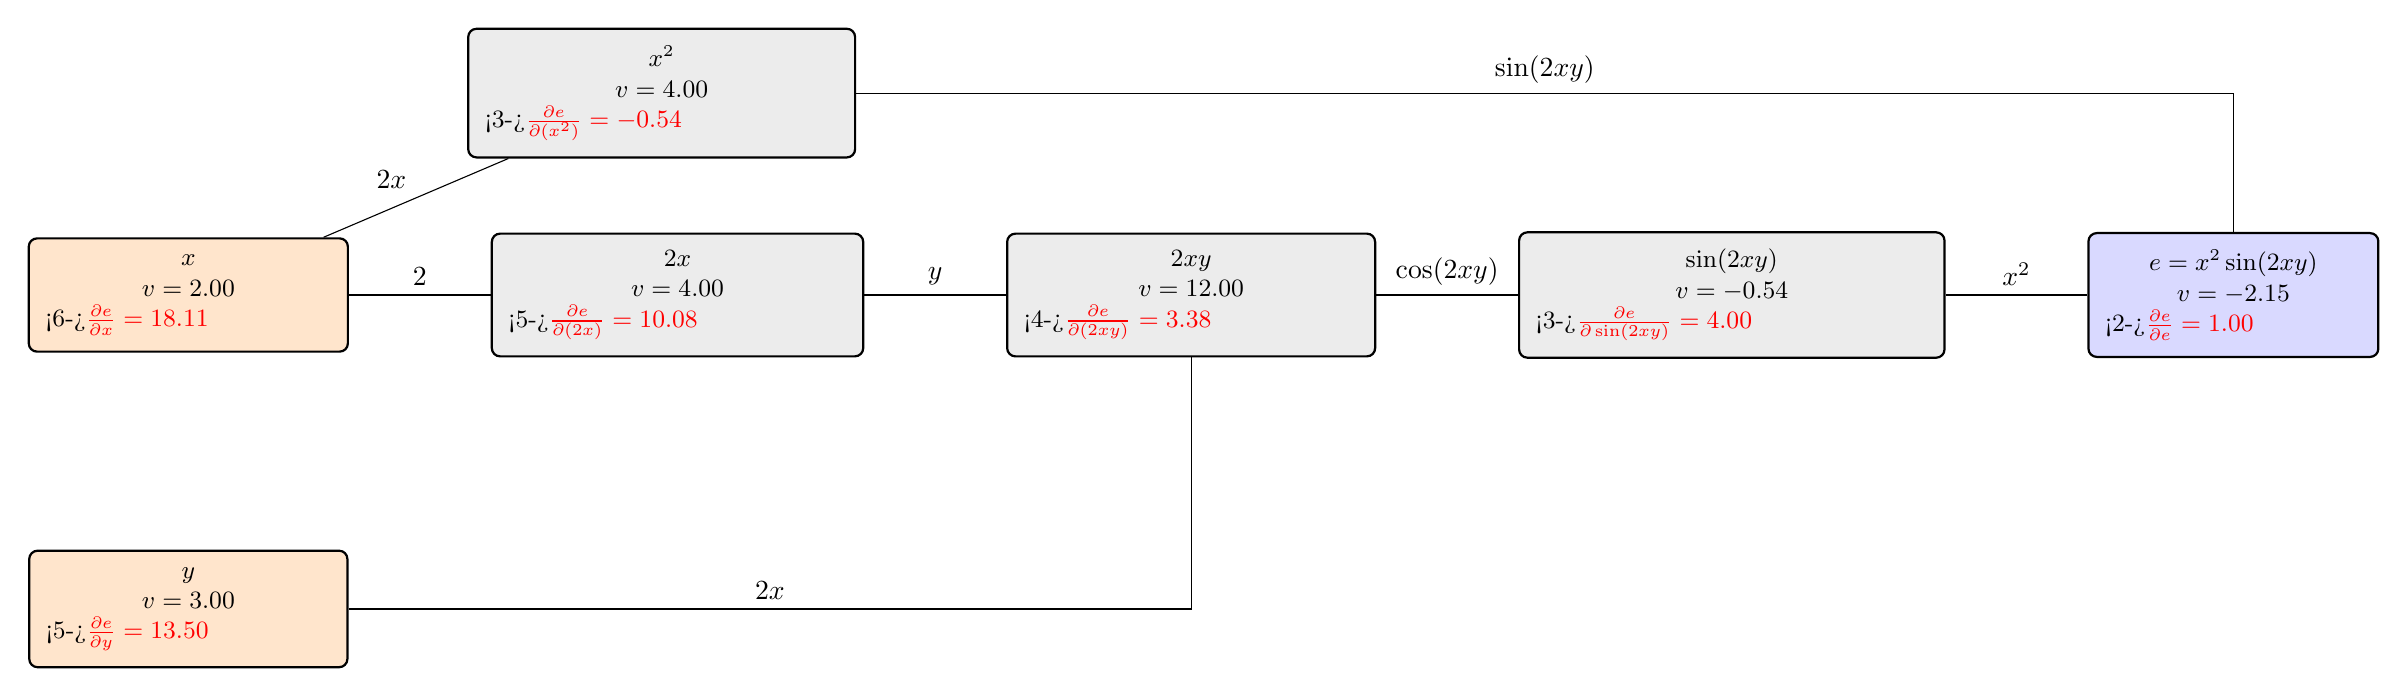
\begin{tikzpicture}[
    node distance=1.5cm and 1.8cm,
    base/.style={draw, rounded corners=3pt, inner sep=6pt, minimum width=1.5cm, align=center, font=\small},
    input/.style={base, draw=black, thick, fill=orange!20},
    op/.style={base, draw=black, thick, fill=gray!15},
    output/.style={base, draw=black, thick, fill=blue!15},
    active/.style={draw=red, very thick},
    fwd/.style={->, draw=black, thick, >={Stealth[scale=1.2]}},
    bwd/.style={<-, draw=red, very thick, >={Stealth[scale=1.3]}},
    lbl inactive/.style={text=black},
    lbl active/.style={text=red, font=\bfseries}
]

% --- Nodes ---
\node[input, alt=<6>{active}{}]
    (x) {$x$ \\ $v=2.00$ \\ \alt<6->{\textcolor{red}{$\frac{\partial e}{\partial x}=18.11$}}{\phantom{$\frac{\partial e}{\partial x}=18.11$}}};

\node[input, alt=<5>{active}{}, below=2.5cm of x]
    (y) {$y$ \\ $v=3.00$ \\ \alt<5->{\textcolor{red}{$\frac{\partial e}{\partial y}=13.50$}}{\phantom{$\frac{\partial e}{\partial y}=13.50$}}};

\node[op, alt=<3>{active}{}, above right=1cm and 1.5cm of x]
    (x2) {$x^2$ \\ $v=4.00$ \\ \alt<3->{\textcolor{red}{$\frac{\partial e}{\partial (x^2)}=-0.54$}}{\phantom{$\frac{\partial e}{\partial (x^2)}=-0.54$}}};

\node[op, alt=<5>{active}{}, right=of x]
    (2x) {$2x$ \\ $v=4.00$ \\ \alt<5->{\textcolor{red}{$\frac{\partial e}{\partial (2x)}=10.08$}}{\phantom{$\frac{\partial e}{\partial (2x)}=10.08$}}};

\node[op, alt=<4>{active}{}, right=of 2x]
    (2xy) {$2xy$ \\ $v=12.00$ \\ \alt<4->{\textcolor{red}{$\frac{\partial e}{\partial (2xy)}=3.38$}}{\phantom{$\frac{\partial e}{\partial (2xy)}=3.38$}}};

\node[op, alt=<3>{active}{}, right=of 2xy]
    (sin) {$\sin(2xy)$ \\ $v=-0.54$ \\ \alt<3->{\textcolor{red}{$\frac{\partial e}{\partial \sin(2xy)}=4.00$}}{\phantom{$\frac{\partial e}{\partial \sin(2xy)}=4.00$}}};

\node[output, alt=<2>{active}{}, right=of sin]
    (final) {$e = x^2 \sin(2xy)$ \\ $v=-2.15$ \\ \alt<2->{\textcolor{red}{$\frac{\partial e}{\partial e}=1.00$}}{\phantom{$\frac{\partial e}{\partial e}=1.00$}}};

% --- Edges (Drawn Forward, Highlighted Backward) ---
\draw[alt=<6>{bwd}{fwd}] (x) -- node[midway, above left, alt=<6>{lbl active}{lbl inactive}] {$2x$} (x2);
\draw[alt=<6>{bwd}{fwd}] (x) -- node[midway, above, alt=<6>{lbl active}{lbl inactive}] {$2$} (2x);
\draw[alt=<5>{bwd}{fwd}] (2x) -- node[midway, above, alt=<5>{lbl active}{lbl inactive}] {$y$} (2xy);
\draw[alt=<5>{bwd}{fwd}] (y) -| node[pos=0.25, above, alt=<5>{lbl active}{lbl inactive}] {$2x$} (2xy);
\draw[alt=<4>{bwd}{fwd}] (2xy) -- node[midway, above, alt=<4>{lbl active}{lbl inactive}] {$\cos(2xy)$} (sin);
\draw[alt=<3>{bwd}{fwd}] (sin) -- node[midway, above, alt=<3>{lbl active}{lbl inactive}] {$x^2$} (final);
\draw[alt=<3>{bwd}{fwd}] (x2) -| node[pos=0.25, above, alt=<3>{lbl active}{lbl inactive}] {$\sin(2xy)$} (final);

\end{tikzpicture}%
}
\end{frame}

\end{document}